\chapter{Proof of Concept and Evaluation}
\label{cap:evaluation}

% Introduction...

In this chapter, we present how the automatic code generation mechanism, proposed in \autoref{cap:code_gen}, was implemented in a fully functional proof of concept. We also describe how we evaluated the gain in performance and ease of development and deployment for users of our Framework.

To facilitate the development of this project and to keep the scope within a defined limit, we did not use P4 compatible switches, instead, we use software emulation to run the P4 code. This enabled us to develop with great efficiency the generation tool and enabled us to test each interaction of the development, making sure the prototype was functional.


% ==============================================================================
%                               IMPLEMENTATION
% ==============================================================================

\section{Prototype Implementation and Deployment}
\label{sec:evaluation:implementation}
% Probably a small section, be careful not to be redundant (max 2 pages)

% 1. Explain how we implemented RNA and the code generation procedure (focando em aspectos mais arquiteturais e tecnologias empregadas. Os *why*s fazem parte do texto até para justificar escolhas mais importantes, mas não são o foco.)

% 2. Explain why we used Python (not that important)

% 3. Explain the master template and the markers (how they are replaced)

% 4. How the code generation is done (using a tree)

% 5. Explain how it is deployed with p4app

In this section, we describe some implementation details of the code generation tool that were not previously discussed. We divide this explanation into three subsections. We first explain the structure of the Protocol and Offloader Templates, which are one of the main inputs for our tool. Then we explain some of the implementation aspects of our prototype. And to finalize, we explain how the output of our tool, the automatically generated code, is deployed in a virtualized network using an emulation of a P4-switch.


\subsection{Protocol and Offloader Templates}

The Protocol and Offloader Templates have a similar structure based on a configuration file. This configuration file is in the Hjson \cite{Hjson} format, which is based on the well-known JSON format. We first explain the Protocol Templates. To explain the Protocol Template's structure, we use the example in Appendix \ref{cap:protocol_template}. Each Protocol Template needs to provide header definitions so it may be parsed. This is done by providing the name of the header structure and the file where it was defined (lines 13 and 12, \autoref{code:icmp_template:config}). The protocols may optionally have a custom \textit{ingress processor} and a custom parser to enable parsing of variable-size headers, both of which were explained in \autoref{sec:rna:detailed_design}.

To enable a Protocol Template to be linked to its children, we need to define the parameter called \texttt{next\_protocol\_selector}. It specifies the field of the protocol's header that will be used to select the next protocol (line 15, \autoref{code:icmp_template:config}). To link a protocol to its parent, we need to specify the parent's protocol identifier (line 7) and specify what value the \texttt{next\_protocol\_selector} must have, for the packet to be forwarded to the child protocol (line 8). With this structure, the mechanism is able to generate all required code for parsing the protocols in the Switch Engine. Each protocol template may have more than one parent.

An Offloader Template is also based on a configuration file, and we use the \autoref{code:icmp_echo:config} as an example. Each protocol needs to be associated with a Protocol Template by its identifier (line 5, \autoref{code:icmp_echo:config}). Each Offloader then must have its own header structure (line 8). This header structure is defined in a P4 file, which is also a part of the template, and its path must be specified in the configuration (line 9). The rest of the parameters used for the Switch Engine are extracted from separate P4 files, the splicer, and the trigger condition (lines 10 and 11). For the Host Engine, the template must specify the C++ code and header files, as well as the name and \textit{namespace} of the Analyzer (lines 14 to 22). To finalize, the configuration also specifies what Zeek Events the Offloader is capable of offloading (lines 23 to 26). Examples for the files of an Offloader Template can be found in Appendix \ref{cap:offloader_template}.

\subsection{Prototype Implementation}

Our prototype implementation of the code generation mechanism follows all architectural details explained in Chapters \ref{cap:rna} and \ref{cap:code_gen}. It was implemented in Python 3 in a modular way so it could be maintained and further developed as the RNA Framework grows. To explain further details of the implementation that were not yet discussed, we follow the same structure used to explain the mechanism details in \autoref{sec:code_gen:detailed}, and we start the Event Extraction part.

The Event Extraction was a very strong point for using Python as our programming language since Zeek provides its own library for parsing Zeek Scripts, which is implemented in Python. In this phase, we parse the provided Zeek Scripts and search their Abstract Syntax Tree (AST) for event handler declarations. Once those event declarations are found, we extract their identifiers and forward this list of identifiers to the next phase, the Knowledge Model Builder.

The Knowledge Model Builder uses as inputs the templates and the Zeek Script events. In this phase, we create a graph structure following the \autoref{alg:build_graph} and procedures explained in the \autoref{sec:code_gen:detailed}. In our implementation, we use exceptions to handle the flow of the algorithm and abort when any requirements are not met. Since our implementation of the Knowledge Model Builder does not differ from the algorithm explained in \autoref{sec:code_gen:detailed}, we do not repeat the explanation in this section.

The Code Generation in our prototype uses template files with markers to insert the generated code in the correct location. The files used for this purpose are called \textit{master template} files and this is what defines the structure and organization of the resulting files. In the \textit{master template}, markers are strings in specific formats that define where a specific code section will be inserted. To generate code that will replace these markers, we use a structure similar to an AST, where each code element is a node, implemented using a class, containing its children nodes. The tool first builds this structure, linking all nodes, then converts the root node to a string. This conversion is done recursively by every node, returning in the end, the full generated code. When the code is generated, we replace all markers with it and save the file to the output directory.

The output of our tool is also composed of code that is provided with each template. To merge these provided sections of code, we use the same strategy as explained in the previous paragraph. We use template files with markers to define where each part of the code will be inserted. We also split some files, mainly on the Zeek Script, as \textit{no-edit} files. These \textit{no-edit} files are copied to the output location as they are, because they do not need any modifications and most of them are static files required by the Zeek Package structure.

When our tool is executed, it generates an output folder containing all the automatically generated code. As explained in the previous chapter, we have not yet implemented the deployment of the P4 code using the Zeek Package, so we split this output folder into two sub-folders. One of the folders contains the P4 code for the switch, and one contains the Zeek Plugin package. In the next section, we explain how the P4 and the Zeek Plugin are deployed.

\subsection{RNA Deployment}
\label{sec:evaluation:deployment}

The deployment of the automatically generated RNA Framework takes place in a virtualized network and using an emulated P4 switch, so no specific hardware or PFDs are required to test our solution. To emulate the switch we use the \textit{p4app} tool, which compiles and runs the P4 code, emulating a programmable forwarding device. To set up this network, the \textit{p4app} uses a tool called \textit{mininet}, which creates all the interfaces for each of our devices and allows us to simulate different network topologies. To run Zeek, we use a custom Docker image that contains all required dependencies. When executed, we link this Docker container's network to the \textit{p4app} container, which allows us to run Zeek on any interfaces of the virtual switch, but usually, on the port setup as a mirroring port.

In our tests, we used a simple topology with two hosts, each one in its own network, with a mirroring port in the switch, where Zeek is listening. The hosts are linked by our switch, which also acts as a router. The mRNA messages generated by the switch are sent to the mirroring port, where Zeek is listening for incoming packets. To generate the traffic that is analyzed by our solution, we used two different methods. The first method is using \textit{p4app} to open terminals in virtual hosts, where we are able to run programs and generate traffic for the Framework to process. The second method is using packet traces that were previously captured and forwarding these traces to be processed as incoming traffic.

% 
% ====================       Pode revisar até aqui :)       ====================
% 


% ==============================================================================
%                                EVALUATION
% ==============================================================================

\section{Evaluation}
\label{sec:evaluation:evaluation}

We now present an evaluation of our proposed solutions, both the RNA and the automatic code generation mechanism. We assess the ability of our code generator to generate correct code and how it enables an inexperienced network operator to offload monitoring scripts to PDPs. Last, we assess the performance of the output of our solution, the automatically generated instance of the RNA Framework. These metrics can be formalized as the following research questions (RQs):

\begin{itemize}
    \item \textit{RQ1}: Is the code generator mechanism able to correctly generate code to offload a set of Zeek Scripts using RNA?
    
    \item \textit{RQ2}: How many lines of code did the code generator generate? And how many extra lines would a developer or network operator need to code to deploy the solution?
    
    \item \textit{RQ3}: How does the performance of a Zeek deployment with RNA compares to a deployment without RNA?
\end{itemize}

To answer those questions, we deploy an automatically generated instance of RNA, and test it using traces containing attacks that trigger warnings on a set of predefined scripts. To limit the scope of this project, we decided that the supported scripts should \textit{(1) not require any state management by the RNA generated code}, and should \textit{(2) not require any stream reassembly}. Those scripts are:

\begin{itemize}
    \item \textit{FTP Bruteforcing}: This script detects FTP authentication brute-force attacks. It triggers a warning after a number of unsuccessful login attempts by a FTP client.
    \item \textit{Detect traceroute}: Detects trace-route attempts by monitoring \textit{ICMP Time Exceeded} messages. This scripts was is provided by Zeek, but due to its usage of \textit{Signature Detection}, which we do not yet support, we set it to only monitor \textit{ICMP Time Exceeded}.
    \item \textit{ICMP Pingback}: Developed by \citeonline{CorelightPingback}, it detects the usage of ICMP ping tunnels created by the Pingback C2 tool.
    \item \textit{NTP Monlist}: Developed by \citeonline{NtpMonlist}, this script detects NTP Monlist attacks.
\end{itemize}


% To evaluate the functionality and performance of our tool we deploy our solution with four different types of monitoring scripts. These scripts are tested with a data-set containing packets 

% Explain objectives (and metrics overview)


\subsection{Experiment data-set}

The data-set used for our experiments was a combination of legitimate packet traces with attack traces generated by us. The legitimate data-set used was the \textit{CAIDA Anonymized Internet Traces 2016} \cite{CAIDA2016}, which was extracted from a high throughput backbone. Since the CAIDA data-set was too big, we selected only a small ten-second window to use for our experiments, which we now refer to as our \textit{legitimate data-set}. This data-set was then merged with smaller well-known or generated attack traces, which we call \textit{attacks data-set}, with $1200$ packets. Combining these two data-sets ensures our previously mentioned scripts will trigger warnings. This combined data-set is the one used for our experiments, which we refer to as the \textit{combined data-set}. The combined data-set has $5.5$ million packets, and an average of $556$ thousand packets per second (kpps) and $3269$ Mega bits per second (Mbps). \autoref{fig:pps_in_time} shows the variation of pps in time for our dataset.

\begin{figure}[htb]
    \caption{Packets Per Second (PPS) in time for the data-set}
    \begin{center}
        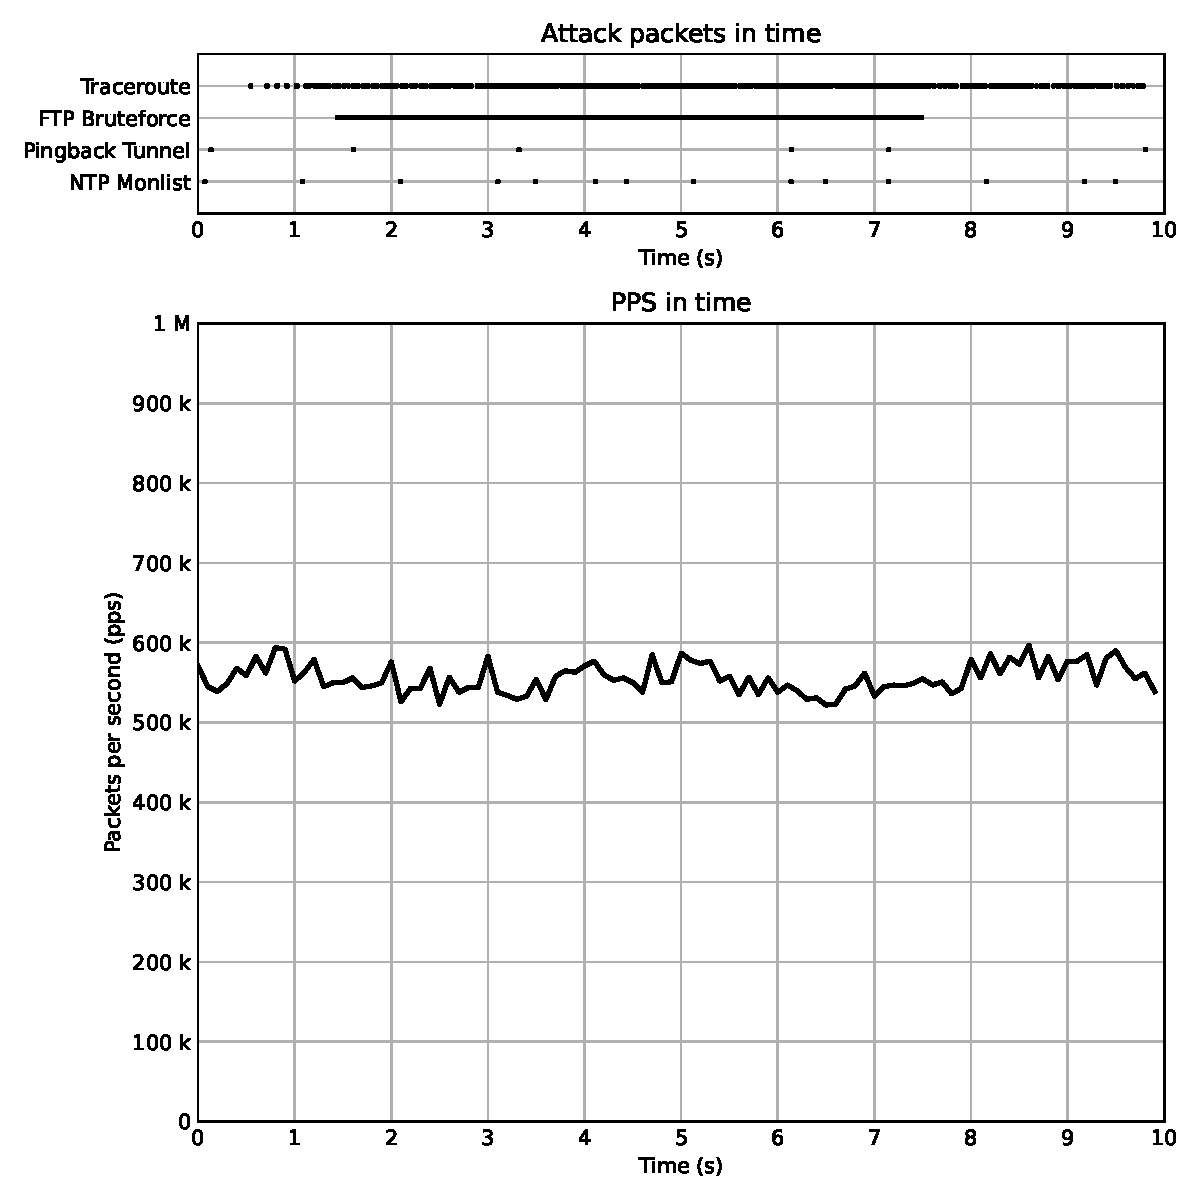
\includegraphics[width=0.7\textwidth]{images/pps_in_time.pdf}  
    \end{center}
    \label{fig:pps_in_time}
    \legend{Source: the author}
\end{figure}

% Explain the data-set (with plots) + attacks + ferramentas para gerar data-set
% - Data-sets status: taxa de pico, pps, total size, duration, packets, caracteristics...
% - Attacks:
% - FTP Bruteforcing
% - Pingback https://github.com/corelight/pingback
% - Detect traceroute
% - NTP Monlist



\subsection{Experiment setup and methodology}
\label{sec:evaluation:setup}

In this section, we describe how we the setup of our experiment. The experiment used the same technologies described in \autoref{sec:evaluation:deployment}, relying on network virtualization, P4 emulation to run our switch, and containerization to run the Zeek. The objective of our evaluation was to compare the functionality and performance of the Zeek Scripts without RNA, compared to with RNA. Since we use emulated switches in our deployments, we assess only the performance of the Zeek monitoring system. We assume that programmable forwarding devices are able to execute the program inline rate if the provided program fits the device's memory.

Switch emulation does not perform as fast as a real hardware P4-switch, which makes it impossible for us to execute our experiment with a P4-switch in real time. In this scenario, the emulated switch would become a bottleneck, preventing the traffic from reaching Zeek at the same rate as it enters the P4 pipeline. To overcome this problem, we process the combined data-set before running the experiment, effectively creating a second data-set. This second data-set represents a real-world output of a P4-switch, receiving our combined data-set and processing it inline rate. We call this second data-set the \textit{RNA data-set}.

To explain the generation this second generate this data-set, we use \autoref{fig:rna_dataset_diagram}. The first step is to select from our data-set only the packets that may trigger an Offloader which will eventually generate a mRNA message. With this intermediate trace, we execute our emulated P4-switch, which is now able to process the data-set faster due to the decreased amount of traffic. This results in a data-set with only mRNA messages, the \textit{RNA data-set}.

\begin{figure}[htb]
    \caption{RNA data-set creation diagram}
    \begin{center}
        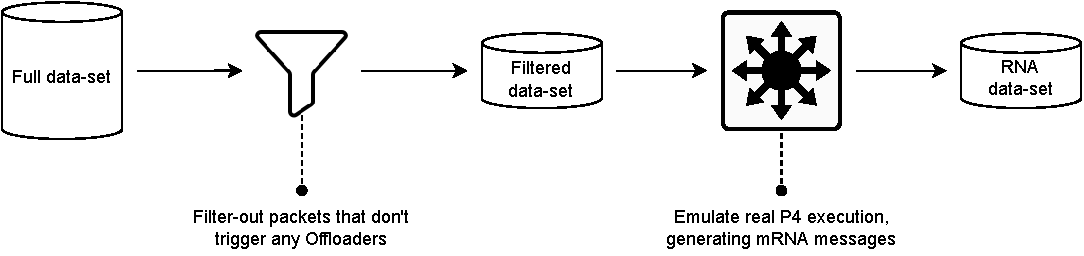
\includegraphics[width=1.0\textwidth]{images/rna_dataset_creation.pdf}  
    \end{center}
    \label{fig:rna_dataset_diagram}
    \legend{Source: the author}
\end{figure}

Now that we have our two data-set, the original one, and the \textit{RNA data-set}, we need to execute Zeek in both scenarios and compare its output and performance. This is done by running Zeek in a Docker container connected to the host computer by a virtual network interface. In this network interface, we replay those two traces, one at a time, and record the memory and CPU usage. Each scenario was executed fifteen times to account for variabilities.

The experiment was executed using a Dell XPS notebook with an Intel Core i9-10885H (8 core, 16 thread) CPU, 16 Gb (2x 8Gb) of DDR4 RAM (3200 MT/s) and a 1 Tb NVMe SSD.

% Methodology?

% \subsection{Methodology}

% Explain results
% - accuracy
%   + script count
% - development cost savings (and less prone to development mistakes)
%   - Show table with multiple combinations of scripts: [1], [2], [3], [4], [1, 2, 3, 4]
% - performance gain
%   - memory, cpu, (execution time/detection time)


\subsection{Results}

In this section we describe the results of our experiment and functional assessment of our code generation mechanism. We first present the functional results, answering research questions one and two, then we present the performance results, answering \textit{RQ3}.

\subsubsection*{Functional results}

To assess whether our proposed mechanism works, we used our prototype and the attacks data-set to compare the output of a Zeek deployment with and one without RNA. After executing both setups and comparing the output of Zeek's \textit{notices}, we conclude that our code generation mechanism was able to generate code to successfully offload four different scripts.

To answer the second question, we manually inspect the generated code for RNA. Our objective is to check whether our solution is helpful and facilitates the deployment of RNA. The generated output instance of RNA for offloading our four Zeek Scripts (described above in this section) has $2966$ lines of code. To develop a new Protocol Template, according to our \autoref{table:lines_by_protocol_template}, an average of $56$ lines of code would need to be written, and for a new Offloader Template (\autoref{table:lines_by_offloader_template}), an average of $240$. This gives developers a big advantage over writing a full standalone solution when any script changes because they do not need to maintain a single code repository, but can manage each individual protocol and Offloader template, and would need to write less code comparing to developing a full solution for each Offloader.

\begin{table}[htb]
    \caption{Lines of code of Protocol Templates}
    \begin{center}
        \begin{tabular}{|l|r|}
            \hline
            Protocol Template & Lines of Code \\ \hline
            Ethernet Protocol & 26           \\ \hline
            IPv4 Protocol     & 43           \\ \hline
            IPv6 Protocol     & 37           \\ \hline
            ICMP Protocol     & 136          \\ \hline
            TCP Protocol      & 67           \\ \hline
            UDP Protocol      & 31           \\ \hline
            \textbf{Total}    & \textbf{340} \\ \hline
        \end{tabular}%
    \end{center}
    \label{table:lines_by_protocol_template}
\end{table}

\begin{table}[htb]
    \caption{Lines of code of Protocol Templates}
    \begin{center}
        \begin{tabular}{|l|r|}
            \hline
            Offloader Template                           & Lines of Code \\ \hline
            NTP Message Offloader                        & 179 \\ \hline
            ICMP Echo Offloader                          & 185 \\ \hline
            ICMP Time Exceeded and Unreachable Offloader & 333 \\ \hline
            FTP Request and Reply Offloader              & 263 \\ \hline
            \textbf{Total}                               & \textbf{960} \\ \hline
        \end{tabular}%
    \end{center}
    \label{table:lines_by_offloader_template}
\end{table}

\subsubsection*{Performance results}

To answer our third research question and assess the performance gain of offloading scripts with RNA, we replayed both of our data-sets, the \textit{combined data-set} and the \textit{RNA data-set}. When replaying the RNA data-set, we enabled our Zeek Plugin, which processed the incoming mRNA messages. This resulted in a significant gain in performance. As Figures \ref{fig:perf_with_rna} and \ref{fig:perf_without_rna} show, the average CPU usage without RNA is $109\%$, and memory usage reaching a maximum of $960.64$ Mb in the end of the experiment, compared to the average $1.9\%$ CPU utilization and maximum of $235.07$ Mb with RNA. Additionally, without RNA an average of $35.24\%$ (median of $35.97\%$) of the packets were dropped. The high dropped packet rate resulted in one of the attacks, the FTP Bruteforce Attack, not been detected in $93.3\%$ of the iterations executed without RNA. Using our solution, no packets were dropped and all attacks were detected in all executions of the experiment.

% Metrics:
% 1. How many scripts we can run (without intervention)
% 2. How many lines were produced per script
%     a. Include copied from the template (maybe create a table with the outline)
% 3. Performance gain in offloading (optional): compare a raw data set vs mRNA messages data set.
%     a. memory, cpu, execution time


% - FTP Bruteforcing (done)
% - Pingback (done): https://github.com/corelight/pingback
% - Detect traceroute (theoretically done)
% - NTP Monlist




\begin{figure}[htb]
    \caption{Performance evaluation with RNA}
    \begin{subfigure}{.5\textwidth}
        \centering
        \vspace{1em}
        \caption{CPU usage by time (with RNA)}
        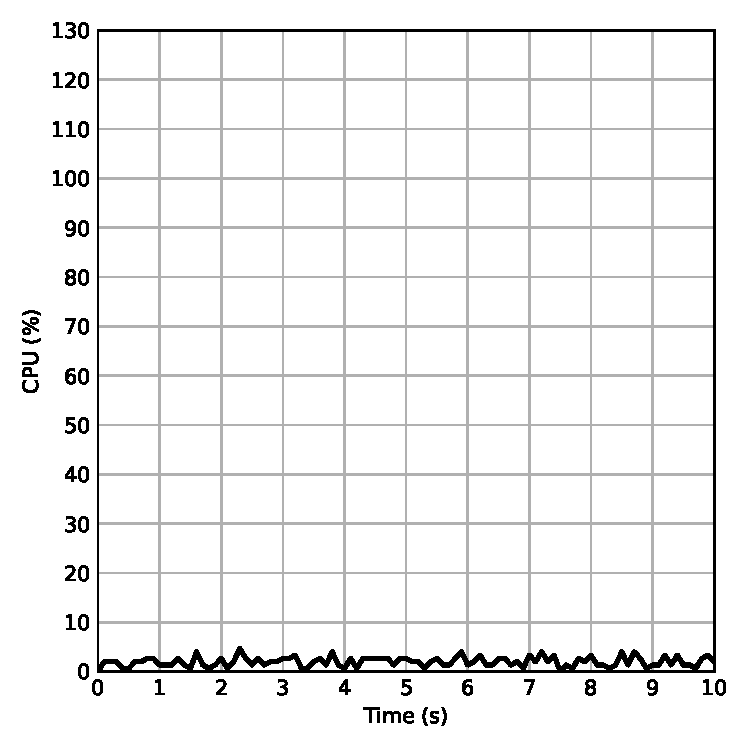
\includegraphics[width=1.0\textwidth]{images/cpu_with_rna.pdf}
    \end{subfigure}%
    \begin{subfigure}{.5\textwidth}
        \centering
        \vspace{1em}
        \caption{Memory usage by time (with RNA)}
        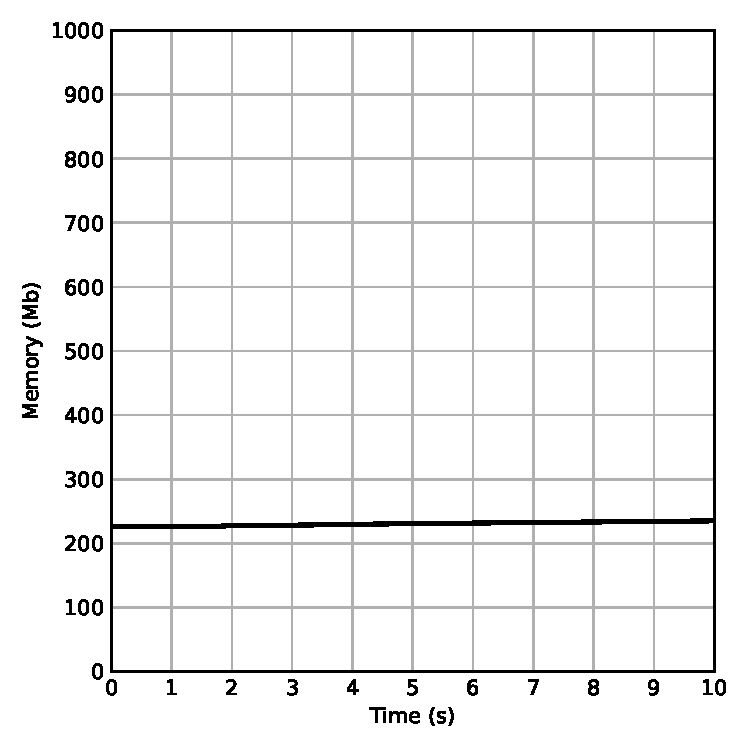
\includegraphics[width=1.0\textwidth]{images/memory_with_rna.pdf}
    \end{subfigure}
    \label{fig:perf_with_rna}
    \legend{Source: author}
\end{figure}

\begin{figure}[htb]
    \caption{Performance evaluation without RNA}
    \begin{subfigure}{.5\textwidth}
        \centering
        \vspace{1em}
        \caption{CPU usage by time (without RNA)}
        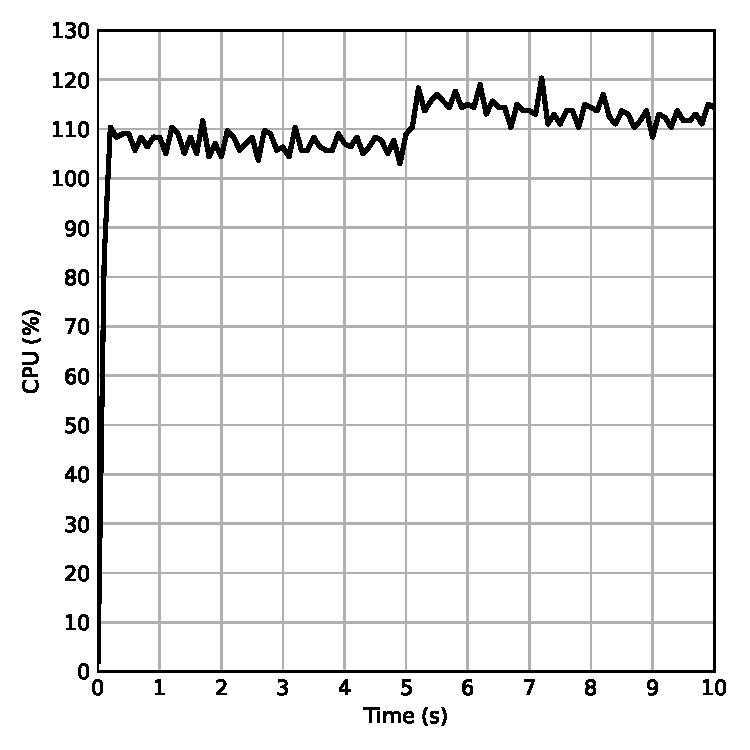
\includegraphics[width=1.0\textwidth]{images/cpu_without_rna.pdf}
    \end{subfigure}%
    \begin{subfigure}{.5\textwidth}
        \centering
        \vspace{1em}
        \caption{Memory usage by time (without RNA)}
        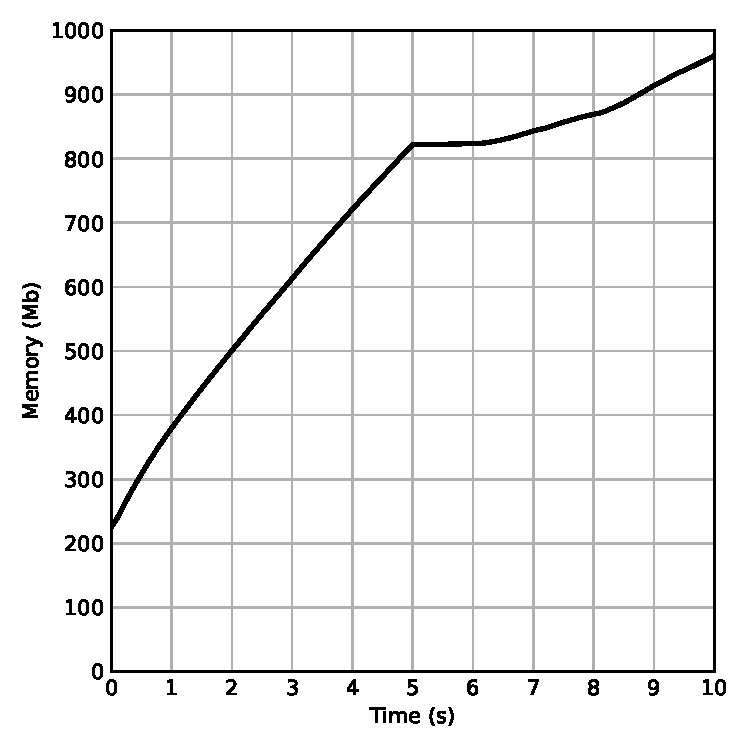
\includegraphics[width=1.0\textwidth]{images/memory_without_rna.pdf}
    \end{subfigure}
    \label{fig:perf_without_rna}
    \legend{Source: author}
\end{figure}
